% Options for packages loaded elsewhere
\PassOptionsToPackage{unicode}{hyperref}
\PassOptionsToPackage{hyphens}{url}
%
\documentclass[
  ignorenonframetext,
]{beamer}
\usepackage{pgfpages}
\setbeamertemplate{caption}[numbered]
\setbeamertemplate{caption label separator}{: }
\setbeamercolor{caption name}{fg=normal text.fg}
\beamertemplatenavigationsymbolsempty
% Prevent slide breaks in the middle of a paragraph
\widowpenalties 1 10000
\raggedbottom
\setbeamertemplate{part page}{
  \centering
  \begin{beamercolorbox}[sep=16pt,center]{part title}
    \usebeamerfont{part title}\insertpart\par
  \end{beamercolorbox}
}
\setbeamertemplate{section page}{
  \centering
  \begin{beamercolorbox}[sep=12pt,center]{part title}
    \usebeamerfont{section title}\insertsection\par
  \end{beamercolorbox}
}
\setbeamertemplate{subsection page}{
  \centering
  \begin{beamercolorbox}[sep=8pt,center]{part title}
    \usebeamerfont{subsection title}\insertsubsection\par
  \end{beamercolorbox}
}
\AtBeginPart{
  \frame{\partpage}
}
\AtBeginSection{
  \ifbibliography
  \else
    \frame{\sectionpage}
  \fi
}
\AtBeginSubsection{
  \frame{\subsectionpage}
}
\usepackage{lmodern}
\usepackage{amssymb,amsmath}
\usepackage{ifxetex,ifluatex}
\ifnum 0\ifxetex 1\fi\ifluatex 1\fi=0 % if pdftex
  \usepackage[T1]{fontenc}
  \usepackage[utf8]{inputenc}
  \usepackage{textcomp} % provide euro and other symbols
\else % if luatex or xetex
  \usepackage{unicode-math}
  \defaultfontfeatures{Scale=MatchLowercase}
  \defaultfontfeatures[\rmfamily]{Ligatures=TeX,Scale=1}
\fi
\usetheme[]{Copenhagen}
\usecolortheme{dolphin}
\usefonttheme{structurebold}
% Use upquote if available, for straight quotes in verbatim environments
\IfFileExists{upquote.sty}{\usepackage{upquote}}{}
\IfFileExists{microtype.sty}{% use microtype if available
  \usepackage[]{microtype}
  \UseMicrotypeSet[protrusion]{basicmath} % disable protrusion for tt fonts
}{}
\makeatletter
\@ifundefined{KOMAClassName}{% if non-KOMA class
  \IfFileExists{parskip.sty}{%
    \usepackage{parskip}
  }{% else
    \setlength{\parindent}{0pt}
    \setlength{\parskip}{6pt plus 2pt minus 1pt}}
}{% if KOMA class
  \KOMAoptions{parskip=half}}
\makeatother
\usepackage{xcolor}
\IfFileExists{xurl.sty}{\usepackage{xurl}}{} % add URL line breaks if available
\IfFileExists{bookmark.sty}{\usepackage{bookmark}}{\usepackage{hyperref}}
\hypersetup{
  pdftitle={Quantitative Hypothesis Test},
  pdfauthor={Alex Sanchez, Miriam Mota, Ricardo Gonzalo and Santiago Perez-Hoyos},
  hidelinks,
  pdfcreator={LaTeX via pandoc}}
\urlstyle{same} % disable monospaced font for URLs
\newif\ifbibliography
\usepackage{color}
\usepackage{fancyvrb}
\newcommand{\VerbBar}{|}
\newcommand{\VERB}{\Verb[commandchars=\\\{\}]}
\DefineVerbatimEnvironment{Highlighting}{Verbatim}{commandchars=\\\{\}}
% Add ',fontsize=\small' for more characters per line
\usepackage{framed}
\definecolor{shadecolor}{RGB}{248,248,248}
\newenvironment{Shaded}{\begin{snugshade}}{\end{snugshade}}
\newcommand{\AlertTok}[1]{\textcolor[rgb]{0.94,0.16,0.16}{#1}}
\newcommand{\AnnotationTok}[1]{\textcolor[rgb]{0.56,0.35,0.01}{\textbf{\textit{#1}}}}
\newcommand{\AttributeTok}[1]{\textcolor[rgb]{0.77,0.63,0.00}{#1}}
\newcommand{\BaseNTok}[1]{\textcolor[rgb]{0.00,0.00,0.81}{#1}}
\newcommand{\BuiltInTok}[1]{#1}
\newcommand{\CharTok}[1]{\textcolor[rgb]{0.31,0.60,0.02}{#1}}
\newcommand{\CommentTok}[1]{\textcolor[rgb]{0.56,0.35,0.01}{\textit{#1}}}
\newcommand{\CommentVarTok}[1]{\textcolor[rgb]{0.56,0.35,0.01}{\textbf{\textit{#1}}}}
\newcommand{\ConstantTok}[1]{\textcolor[rgb]{0.00,0.00,0.00}{#1}}
\newcommand{\ControlFlowTok}[1]{\textcolor[rgb]{0.13,0.29,0.53}{\textbf{#1}}}
\newcommand{\DataTypeTok}[1]{\textcolor[rgb]{0.13,0.29,0.53}{#1}}
\newcommand{\DecValTok}[1]{\textcolor[rgb]{0.00,0.00,0.81}{#1}}
\newcommand{\DocumentationTok}[1]{\textcolor[rgb]{0.56,0.35,0.01}{\textbf{\textit{#1}}}}
\newcommand{\ErrorTok}[1]{\textcolor[rgb]{0.64,0.00,0.00}{\textbf{#1}}}
\newcommand{\ExtensionTok}[1]{#1}
\newcommand{\FloatTok}[1]{\textcolor[rgb]{0.00,0.00,0.81}{#1}}
\newcommand{\FunctionTok}[1]{\textcolor[rgb]{0.00,0.00,0.00}{#1}}
\newcommand{\ImportTok}[1]{#1}
\newcommand{\InformationTok}[1]{\textcolor[rgb]{0.56,0.35,0.01}{\textbf{\textit{#1}}}}
\newcommand{\KeywordTok}[1]{\textcolor[rgb]{0.13,0.29,0.53}{\textbf{#1}}}
\newcommand{\NormalTok}[1]{#1}
\newcommand{\OperatorTok}[1]{\textcolor[rgb]{0.81,0.36,0.00}{\textbf{#1}}}
\newcommand{\OtherTok}[1]{\textcolor[rgb]{0.56,0.35,0.01}{#1}}
\newcommand{\PreprocessorTok}[1]{\textcolor[rgb]{0.56,0.35,0.01}{\textit{#1}}}
\newcommand{\RegionMarkerTok}[1]{#1}
\newcommand{\SpecialCharTok}[1]{\textcolor[rgb]{0.00,0.00,0.00}{#1}}
\newcommand{\SpecialStringTok}[1]{\textcolor[rgb]{0.31,0.60,0.02}{#1}}
\newcommand{\StringTok}[1]{\textcolor[rgb]{0.31,0.60,0.02}{#1}}
\newcommand{\VariableTok}[1]{\textcolor[rgb]{0.00,0.00,0.00}{#1}}
\newcommand{\VerbatimStringTok}[1]{\textcolor[rgb]{0.31,0.60,0.02}{#1}}
\newcommand{\WarningTok}[1]{\textcolor[rgb]{0.56,0.35,0.01}{\textbf{\textit{#1}}}}
\setlength{\emergencystretch}{3em} % prevent overfull lines
\providecommand{\tightlist}{%
  \setlength{\itemsep}{0pt}\setlength{\parskip}{0pt}}
\setcounter{secnumdepth}{-\maxdimen} % remove section numbering

\title{Quantitative Hypothesis Test}
\author{Alex Sanchez, Miriam Mota, Ricardo Gonzalo and\\
Santiago Perez-Hoyos}
\date{Statistics and Bioinformatics Unit. Vall d'Hebron Institut de Recerca
14/10/2020}

\begin{document}
\frame{\titlepage}

\begin{frame}[fragile]

\tiny

\begin{Shaded}
\begin{Highlighting}[]
\NormalTok{oldpar<-}\KeywordTok{par}\NormalTok{(}\DataTypeTok{mfrow=}\KeywordTok{c}\NormalTok{(}\DecValTok{1}\NormalTok{,}\DecValTok{1}\NormalTok{)) }\CommentTok{# Guarda los parámetros para el dibgujo}
\KeywordTok{par}\NormalTok{(}\DataTypeTok{mfrow=}\KeywordTok{c}\NormalTok{(}\DecValTok{2}\NormalTok{,}\DecValTok{2}\NormalTok{)) }\CommentTok{# Dibuja cuatro gráficos por grafico}
\KeywordTok{with}\NormalTok{(hta, }\KeywordTok{boxplot}\NormalTok{(tas1, }\DataTypeTok{main=}\StringTok{"Box-plot"}\NormalTok{) )}

\KeywordTok{with}\NormalTok{(hta, }\KeywordTok{hist}\NormalTok{(tas1) )}

\KeywordTok{with}\NormalTok{(hta, }\KeywordTok{qqnorm}\NormalTok{(tas1, }\DataTypeTok{main=}\StringTok{"Normal QQplot"}\NormalTok{) );}\KeywordTok{with}\NormalTok{(hta, }\KeywordTok{qqline}\NormalTok{(tas1) )}

\KeywordTok{par}\NormalTok{(oldpar) }\CommentTok{# Vuelve a los parámetros de dibujo originales}
\end{Highlighting}
\end{Shaded}

\begin{figure}
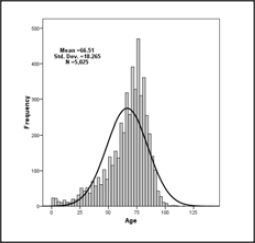
\includegraphics[width=0.8\linewidth]{images/normalityplot} \end{figure}

\end{frame}

\begin{frame}[fragile]{Normality Test}
\protect\hypertarget{normality-test}{}

\small

\begin{Shaded}
\begin{Highlighting}[]
\KeywordTok{with}\NormalTok{(hta,}\KeywordTok{shapiro.test}\NormalTok{(tad1) ) }\CommentTok{# Shapiro Wilk test}
\end{Highlighting}
\end{Shaded}

\begin{verbatim}
## 
##  Shapiro-Wilk normality test
## 
## data:  tad1
## W = 0.96622, p-value = 0.09512
\end{verbatim}

\end{frame}

\begin{frame}[fragile]{One sample Test}
\protect\hypertarget{one-sample-test}{}

\small

\begin{Shaded}
\begin{Highlighting}[]
\KeywordTok{with}\NormalTok{(hta,}\KeywordTok{t.test}\NormalTok{(tad1,}\DataTypeTok{mu=}\DecValTok{90}\NormalTok{) ) }\CommentTok{# One sample T.test}
\end{Highlighting}
\end{Shaded}

\begin{verbatim}
## 
##  One Sample t-test
## 
## data:  tad1
## t = -1.2137, df = 59, p-value = 0.2297
## alternative hypothesis: true mean is not equal to 90
## 95 percent confidence interval:
##  85.80626 91.02707
## sample estimates:
## mean of x 
##  88.41667
\end{verbatim}

\end{frame}

\begin{frame}[fragile]{Homogeneity variance Test}
\protect\hypertarget{homogeneity-variance-test}{}

\small

\begin{Shaded}
\begin{Highlighting}[]
\KeywordTok{library}\NormalTok{(car)}
\NormalTok{hta}\OperatorTok\StringTok{ }
\StringTok{  }\KeywordTok{group_by}\NormalTok{(sexo) }\OperatorTok\StringTok{ }
\StringTok{  }\KeywordTok{summarise}\NormalTok{(}\DataTypeTok{var =} \KeywordTok{sd}\NormalTok{(tas1)) }
\end{Highlighting}
\end{Shaded}

\begin{verbatim}
## # A tibble: 2 x 2
##   sexo    var
##   <chr> <dbl>
## 1 MUJER  17.6
## 2 VARON  22.1
\end{verbatim}

\begin{Shaded}
\begin{Highlighting}[]
\KeywordTok{with}\NormalTok{(hta,}\KeywordTok{leveneTest}\NormalTok{(tad1}\OperatorTok{~}\KeywordTok{factor}\NormalTok{(sexo),}\DataTypeTok{center=}\StringTok{"median"}\NormalTok{))}
\end{Highlighting}
\end{Shaded}

\begin{verbatim}
## Levene's Test for Homogeneity of Variance (center = "median")
##       Df F value Pr(>F)
## group  1  1.3506 0.2499
##       58
\end{verbatim}

\begin{itemize}
\tightlist
\item
  p value is over 0.05
\item
  We can assume homogeneity of variances
\end{itemize}

\end{frame}

\begin{frame}[fragile]{T test when variances are equal}
\protect\hypertarget{t-test-when-variances-are-equal}{}

\small

\begin{Shaded}
\begin{Highlighting}[]
\KeywordTok{with}\NormalTok{(hta,}\KeywordTok{t.test}\NormalTok{(tas1}\OperatorTok{~}\KeywordTok{factor}\NormalTok{(sexo),}\DataTypeTok{var.equal=}\OtherTok{TRUE}\NormalTok{ ))}
\end{Highlighting}
\end{Shaded}

\begin{verbatim}
## 
##  Two Sample t-test
## 
## data:  tas1 by factor(sexo)
## t = -0.2471, df = 58, p-value = 0.8057
## alternative hypothesis: true difference in means is not equal to 0
## 95 percent confidence interval:
##  -11.603461   9.053519
## sample estimates:
## mean in group MUJER mean in group VARON 
##            149.5946            150.8696
\end{verbatim}

\begin{itemize}
\tightlist
\item
  Type I Error is over than 0.05
\item
  We cannot reject mean equality
\end{itemize}

\end{frame}

\begin{frame}[fragile]{T test when variances are unequal}
\protect\hypertarget{t-test-when-variances-are-unequal}{}

\small

\begin{Shaded}
\begin{Highlighting}[]
\KeywordTok{with}\NormalTok{(hta,}\KeywordTok{t.test}\NormalTok{(tas1}\OperatorTok{~}\KeywordTok{factor}\NormalTok{(sexo),}\DataTypeTok{var.equal=}\OtherTok{FALSE}\NormalTok{ ))}
\end{Highlighting}
\end{Shaded}

\begin{verbatim}
## 
##  Welch Two Sample t-test
## 
## data:  tas1 by factor(sexo)
## t = -0.23436, df = 39.098, p-value = 0.8159
## alternative hypothesis: true difference in means is not equal to 0
## 95 percent confidence interval:
##  -12.277927   9.727986
## sample estimates:
## mean in group MUJER mean in group VARON 
##            149.5946            150.8696
\end{verbatim}

\begin{itemize}
\tightlist
\item
  Same conclusions as before
\item
  Test is also known as Welch test
\end{itemize}

\end{frame}

\begin{frame}[fragile]{U Mann-Whitney or Sum Rank non parametric test}
\protect\hypertarget{u-mann-whitney-or-sum-rank-non-parametric-test}{}

\small

\begin{Shaded}
\begin{Highlighting}[]
\KeywordTok{with}\NormalTok{(hta,}\KeywordTok{wilcox.test}\NormalTok{(tad1}\OperatorTok{~}\KeywordTok{factor}\NormalTok{(sexo)}
\NormalTok{    ,}\DataTypeTok{alternative=}\StringTok{'two.sided'}\NormalTok{,}\DataTypeTok{exact=}\OtherTok{TRUE}\NormalTok{, }\DataTypeTok{correct=}\OtherTok{FALSE}\NormalTok{))}
\end{Highlighting}
\end{Shaded}

\begin{verbatim}
## 
##  Wilcoxon rank sum test
## 
## data:  tad1 by factor(sexo)
## W = 434, p-value = 0.8955
## alternative hypothesis: true location shift is not equal to 0
\end{verbatim}

\begin{Shaded}
\begin{Highlighting}[]
\NormalTok{hta}\OperatorTok\StringTok{ }
\StringTok{  }\KeywordTok{group_by}\NormalTok{(sexo) }\OperatorTok\StringTok{ }
\StringTok{  }\KeywordTok{summarise}\NormalTok{(}\DataTypeTok{median =} \KeywordTok{median}\NormalTok{(tad1)) }
\end{Highlighting}
\end{Shaded}

\begin{verbatim}
## # A tibble: 2 x 2
##   sexo  median
##   <chr>  <dbl>
## 1 MUJER     90
## 2 VARON     90
\end{verbatim}

\begin{itemize}
\tightlist
\item
  Null Hypothesis cannot be rejected
\end{itemize}

\end{frame}

\begin{frame}[fragile]{Paired T-test}
\protect\hypertarget{paired-t-test}{}

\small

\begin{Shaded}
\begin{Highlighting}[]
\KeywordTok{with}\NormalTok{(hta,}\KeywordTok{t.test}\NormalTok{(tas1,tas12,}\DataTypeTok{paired=}\OtherTok{TRUE}\NormalTok{))}
\end{Highlighting}
\end{Shaded}

\begin{verbatim}
## 
##  Paired t-test
## 
## data:  tas1 and tas12
## t = 6.0672, df = 51, p-value = 1.609e-07
## alternative hypothesis: true difference in means is not equal to 0
## 95 percent confidence interval:
##   8.518285 16.943253
## sample estimates:
## mean of the differences 
##                12.73077
\end{verbatim}

\begin{Shaded}
\begin{Highlighting}[]
\KeywordTok{summary}\NormalTok{(hta}\OperatorTok{$}\NormalTok{tas1)}
\end{Highlighting}
\end{Shaded}

\begin{verbatim}
##    Min. 1st Qu.  Median    Mean 3rd Qu.    Max. 
##   100.0   140.0   145.0   150.1   160.0   210.0
\end{verbatim}

\begin{Shaded}
\begin{Highlighting}[]
\KeywordTok{summary}\NormalTok{(hta}\OperatorTok{$}\NormalTok{tas12)}
\end{Highlighting}
\end{Shaded}

\begin{verbatim}
##    Min. 1st Qu.  Median    Mean 3rd Qu.    Max.    NA's 
##   110.0   130.0   139.0   137.2   150.0   175.0       8
\end{verbatim}

\begin{itemize}
\tightlist
\item
  P value is over 0.05
\end{itemize}

\end{frame}

\begin{frame}[fragile]{Paired Sign-Rank Wilcoxon Test}
\protect\hypertarget{paired-sign-rank-wilcoxon-test}{}

\small

\begin{Shaded}
\begin{Highlighting}[]
\KeywordTok{with}\NormalTok{(hta,}\KeywordTok{wilcox.test}\NormalTok{(tad1,tad12,}
     \DataTypeTok{exact=}\OtherTok{TRUE}\NormalTok{, }\DataTypeTok{paired=}\OtherTok{TRUE}\NormalTok{))}
\end{Highlighting}
\end{Shaded}

\begin{verbatim}
## 
##  Wilcoxon signed rank test with continuity correction
## 
## data:  tad1 and tad12
## V = 478.5, p-value = 0.05333
## alternative hypothesis: true location shift is not equal to 0
\end{verbatim}

\end{frame}

\begin{frame}[fragile]{Read diabetes data}
\protect\hypertarget{read-diabetes-data}{}

\tiny

\begin{Shaded}
\begin{Highlighting}[]
\KeywordTok{library}\NormalTok{(readxl)}
\KeywordTok{library}\NormalTok{(dplyr)}
\KeywordTok{library}\NormalTok{(magrittr)}
\NormalTok{diabetes <-}\StringTok{ }\KeywordTok{read_excel}\NormalTok{(}\StringTok{"datasets/diabetes.xls"}\NormalTok{)}
\KeywordTok{sapply}\NormalTok{(diabetes, class)}
\end{Highlighting}
\end{Shaded}

\begin{verbatim}
##    numpacie        mort    tempsviu        edat         bmi    edatdiag 
##   "numeric" "character"   "numeric"   "numeric"   "numeric"   "numeric" 
##       tabac         sbp         dbp         ecg         chd 
## "character"   "numeric"   "numeric" "character" "character"
\end{verbatim}

\begin{Shaded}
\begin{Highlighting}[]
\NormalTok{diabetes_factor <-}\StringTok{ }\NormalTok{diabetes }\OperatorTok
\StringTok{  }\KeywordTok{mutate_if}\NormalTok{(}\KeywordTok{sapply}\NormalTok{(diabetes, is.character), as.factor) }\OperatorTok
\StringTok{  }\KeywordTok{select}\NormalTok{ (}\OperatorTok{-}\NormalTok{numpacie)}

\NormalTok{diabetes}\OperatorTok\StringTok{ }
\StringTok{  }\KeywordTok{group_by}\NormalTok{(ecg) }\OperatorTok\StringTok{ }
\StringTok{  }\KeywordTok{summarise}\NormalTok{( }\DataTypeTok{n=}\KeywordTok{n}\NormalTok{(),}
    \DataTypeTok{mean =} \KeywordTok{mean}\NormalTok{(edat),}
            \DataTypeTok{sd=}\KeywordTok{sd}\NormalTok{(edat)) }
\end{Highlighting}
\end{Shaded}

\begin{verbatim}
## # A tibble: 3 x 4
##   ecg          n  mean    sd
##   <chr>    <int> <dbl> <dbl>
## 1 Anormal     11  64.9  6.76
## 2 Frontera    27  53.8 11.4 
## 3 Normal     111  50.5 11.5
\end{verbatim}

\end{frame}

\begin{frame}[fragile]{ANOVA}
\protect\hypertarget{anova}{}

\begin{Shaded}
\begin{Highlighting}[]
\NormalTok{anova<-}\KeywordTok{aov}\NormalTok{(edat}\OperatorTok{~}\NormalTok{ecg,}\DataTypeTok{data=}\NormalTok{diabetes_factor)}
\KeywordTok{summary}\NormalTok{(anova)}
\end{Highlighting}
\end{Shaded}

\begin{verbatim}
##              Df Sum Sq Mean Sq F value  Pr(>F)    
## ecg           2   2166  1083.0   8.619 0.00029 ***
## Residuals   146  18347   125.7                    
## ---
## Signif. codes:  0 '***' 0.001 '**' 0.01 '*' 0.05 '.' 0.1 ' ' 1
\end{verbatim}

\end{frame}

\begin{frame}[fragile]{Multicomparison}
\protect\hypertarget{multicomparison}{}

\tiny

\begin{Shaded}
\begin{Highlighting}[]
\KeywordTok{library}\NormalTok{(multcomp)}
\NormalTok{tuk <-}\StringTok{ }\KeywordTok{glht}\NormalTok{(anova, }\DataTypeTok{linfct =} \KeywordTok{mcp}\NormalTok{(}\DataTypeTok{ecg =} \StringTok{"Tukey"}\NormalTok{))}

  \KeywordTok{print}\NormalTok{(}\KeywordTok{summary}\NormalTok{(tuk)) }\CommentTok{# pairwise tests}
\end{Highlighting}
\end{Shaded}

\begin{verbatim}
## 
##   Simultaneous Tests for General Linear Hypotheses
## 
## Multiple Comparisons of Means: Tukey Contrasts
## 
## 
## Fit: aov(formula = edat ~ ecg, data = diabetes_factor)
## 
## Linear Hypotheses:
##                         Estimate Std. Error t value Pr(>|t|)    
## Frontera - Anormal == 0  -11.094      4.010  -2.767 0.016508 *  
## Normal - Anormal == 0    -14.405      3.543  -4.065 0.000228 ***
## Normal - Frontera == 0    -3.310      2.405  -1.376 0.345704    
## ---
## Signif. codes:  0 '***' 0.001 '**' 0.01 '*' 0.05 '.' 0.1 ' ' 1
## (Adjusted p values reported -- single-step method)
\end{verbatim}

\end{frame}

\begin{frame}[fragile]

\tiny

\begin{Shaded}
\begin{Highlighting}[]
  \KeywordTok{print}\NormalTok{(}\KeywordTok{confint}\NormalTok{(tuk, }\DataTypeTok{level=}\FloatTok{0.95}\NormalTok{)) }\CommentTok{# confidence intervals}
\end{Highlighting}
\end{Shaded}

\begin{verbatim}
## 
##   Simultaneous Confidence Intervals
## 
## Multiple Comparisons of Means: Tukey Contrasts
## 
## 
## Fit: aov(formula = edat ~ ecg, data = diabetes_factor)
## 
## Quantile = 2.3463
## 95% family-wise confidence level
##  
## 
## Linear Hypotheses:
##                         Estimate lwr      upr     
## Frontera - Anormal == 0 -11.0943 -20.5022  -1.6864
## Normal - Anormal == 0   -14.4046 -22.7184  -6.0908
## Normal - Frontera == 0   -3.3103  -8.9541   2.3335
\end{verbatim}

\end{frame}

\begin{frame}[fragile]{Multicomparison plot}
\protect\hypertarget{multicomparison-plot}{}

\small

\begin{Shaded}
\begin{Highlighting}[]
  \KeywordTok{plot}\NormalTok{(}\KeywordTok{confint}\NormalTok{(tuk))}
\end{Highlighting}
\end{Shaded}

\end{frame}

\begin{frame}[fragile]{Kruskal-Wallis Test}
\protect\hypertarget{kruskal-wallis-test}{}

\small

\begin{Shaded}
\begin{Highlighting}[]
\NormalTok{diabetes_factor}\OperatorTok\StringTok{ }
\StringTok{  }\KeywordTok{group_by}\NormalTok{(ecg) }\OperatorTok\StringTok{ }
\StringTok{  }\KeywordTok{summarise}\NormalTok{(}\DataTypeTok{median =} \KeywordTok{median}\NormalTok{(edat)) }
\end{Highlighting}
\end{Shaded}

\begin{verbatim}
## # A tibble: 3 x 2
##   ecg      median
##   <fct>     <dbl>
## 1 Anormal      64
## 2 Frontera     53
## 3 Normal       49
\end{verbatim}

\begin{Shaded}
\begin{Highlighting}[]
\KeywordTok{kruskal.test}\NormalTok{(edat}\OperatorTok{~}\NormalTok{ecg,}\DataTypeTok{data=}\NormalTok{diabetes_factor)}
\end{Highlighting}
\end{Shaded}

\begin{verbatim}
## 
##  Kruskal-Wallis rank sum test
## 
## data:  edat by ecg
## Kruskal-Wallis chi-squared = 17.483, df = 2, p-value = 0.0001598
\end{verbatim}

\end{frame}

\begin{frame}[fragile]{Dunn Test for multiple comparison}
\protect\hypertarget{dunn-test-for-multiple-comparison}{}

\small

\begin{Shaded}
\begin{Highlighting}[]
\KeywordTok{library}\NormalTok{(dunn.test)}
\KeywordTok{with}\NormalTok{(diabetes_factor,}\KeywordTok{dunn.test}\NormalTok{(edat,ecg,}\DataTypeTok{method=}\StringTok{"bonferroni"}\NormalTok{))}
\end{Highlighting}
\end{Shaded}

\begin{verbatim}
##   Kruskal-Wallis rank sum test
## 
## data: edat and ecg
## Kruskal-Wallis chi-squared = 17.4826, df = 2, p-value = 0
## 
## 
##                            Comparison of edat by ecg                           
##                                  (Bonferroni)                                  
## Col Mean-|
## Row Mean |    Anormal   Frontera
## ---------+----------------------
## Frontera |   2.721182
##          |    0.0098*
##          |
##   Normal |   4.075469   1.467464
##          |    0.0001*     0.2134
## 
## alpha = 0.05
## Reject Ho if p <= alpha/2
\end{verbatim}

\end{frame}

\end{document}
